\documentclass{article}
\usepackage[margin=0.5in]{geometry}
\usepackage{graphicx}
\usepackage{multirow}
\usepackage{subcaption}
\title{\Huge Assignment 8-Multilevel Queue Scheduling}
\author{22000021}
\date{\today}
 
\begin{document}
\maketitle
\newpage

\section{Introduction}
This program aims to simulate a multilevel queue scheduling algorithm, a crucial aspect of operating system design, where processes are organized into priority-based queues. With four distinct queues assigned priorities from q0 to q3, the algorithm employs different scheduling strategies tailored to each queue's priority level. Specifically, Round Robin (RR) scheduling is used for q0, while Shortest Job First (SJF) scheduling is employed for q1 and q2, and First-In-First-Out (FIFO) scheduling for q3. Each queue is allocated a time quantum of 20 seconds, after which the CPU switches between queues. The program prompts users to input the number of processes and their respective priorities for each queue, facilitating dynamic simulation scenarios. Through this simulation, we aim to analyze the efficiency and performance of various scheduling algorithms under differing workload conditions, providing valuable insights for optimizing system scheduling strategies.


\section{Methodology}
\vspace{\baselineskip}
In this section, we will examine the implementation details of the algorithm.

\subsection{Process Implementation}
\vspace{\baselineskip}
The multilevel queue scheduling algorithm is implemented using \textbf{C++}’s class-based approach.
The ’Process’ structure represents a process with properties such as process ID, burst time, remaining time, wait time Turnaround time. 
The ’Queue’ structure represents a queue with properties such as front, rear, and an array to hold the processes
For the implementation purpose, I have used the maximum number of processes in the queue as 100

\begin{figure}[h]
    \centering
    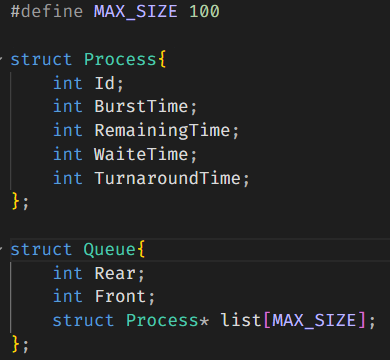
\includegraphics[width=0.6\textwidth,]{1.png}
    \caption{Structures}
    \label{fig:example}
\end{figure}

\newpage
\subsection{Queue Operations}
\vspace{\baselineskip}
The queue operations such as enqueue, dequeue, and checking if the queue is empty or full are implemented as functions.
The scheduling algorithms for each queue are implemented as separate functions.
The the functions IsFull and IsEmpty returns true or false and the Enqueue and Dequeue operation do the inserting and deletion in the queue

\begin{figure}[h!]
    \centering
    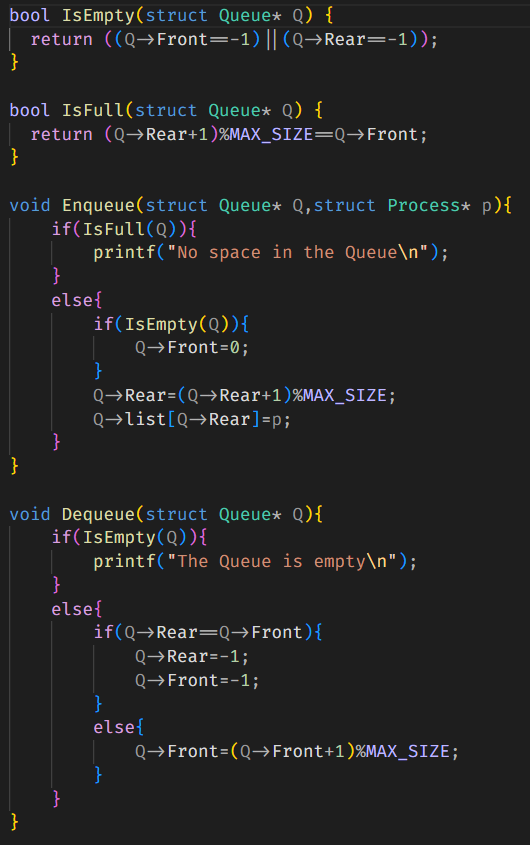
\includegraphics[width=0.5\textwidth,]{2.png}
\end{figure}
\begin{figure}[h!]
    \centering
    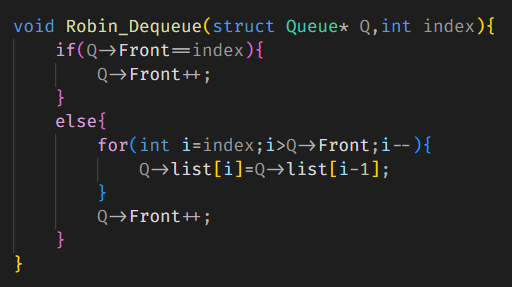
\includegraphics[width=0.5\textwidth,]{3.png}
    \caption{Queue}
    \label{fig:nw}
\end{figure}

\newpage
Enqueue and Dequeue are the same operations following a circular queue.delete is a variation of dequeue, where the dequeued process will be enqueued to the same queue.

\vspace{\baselineskip}
\subsection{Process initialization}
\vspace{\baselineskip}

For the code to work without any interrupts we ask for the user to enter the count of the process that will be processed In c++ we cant do that without user inputs 
The code for initialization of the process after the detail for the process has been input we store the process temporarily to a user define variable and than that process is added to the corresponding queue

\vspace{\baselineskip}
\begin{figure}[h!]
    \centering
    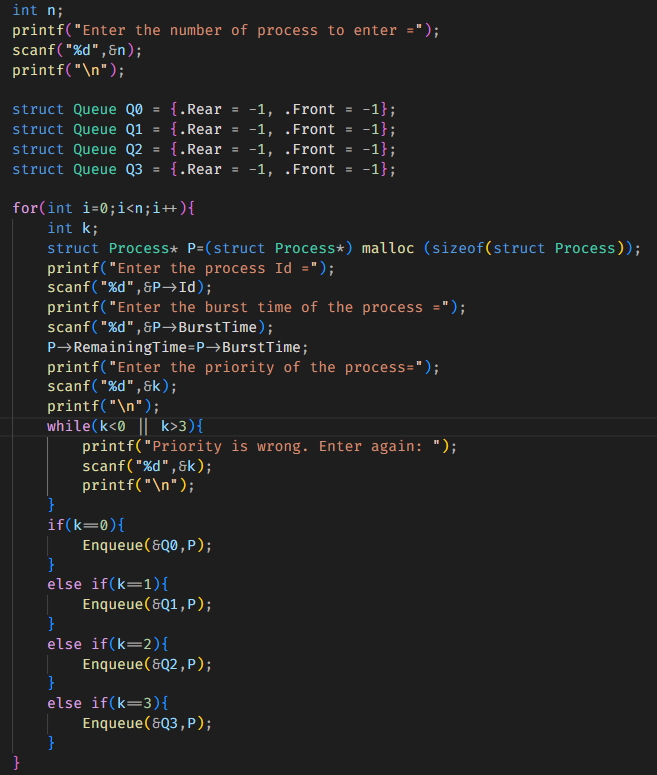
\includegraphics[width=0.8\textwidth]{4.png}
    \caption{Queue}
    \label{fig:ne}
\end{figure}

\newpage
This part of the code initializes four separate queues (Q0, Q1, Q2, and Q3) representing different priority levels in a multilevel queue scheduling algorithm. It first prompts the user to input the number of processes to enter. Then, it iterates n times to input details for each process, such as process ID, burst time, and priority.
During each iteration, memory is dynamically allocated for a new Process. The user is prompted to enter the process details, and the entered information is assigned to the respective members of the Process.
The priority of the process is checked to ensure it falls within the valid range of 0 to 3. If the priority is valid, the process is enqueued into the corresponding queue (Q0, Q1, Q2, or Q3) using the Enqueue() function.
Overall, this section of the code facilitates the dynamic creation and enqueuing of processes into their respective priority-based queues based on user input.

\vspace{\baselineskip}
\section{Scheduling Algorithm}
\vspace{\baselineskip}
\subsection{RR (Round Robin) Scheduling Algorithm}
\begin{itemize}
    \item The function determines the quantum slice by dividing the total number of processes in the queue by the time quantum of the multilevel queue. This ensures fair distribution of time among processes.
    \item if the processes in the queue is greater than 20 seconds we cant use decimal time to execute a process there is a exception when that happens
    \item It enters a loop that iterates until the quantum slice is exhausted. This loop handles cases where the quantum slice is smaller than the Robin slice or vice versa.
    \item If a process's remaining time is less than or equal to the Robin slice, the process completes its execution. It is removed from the queue, and the global time is updated. A message indicating the process ID and exit time is printed
    \item If a process's remaining time exceeds the Robin slice, the Robin slice is subtracted from its remaining time, and the global time is updated accordingly. The process remains in the queue for further execution
    \item This process continues until the quantum slice is exhausted or the queue becomes empty.
\end{itemize}

\vspace{\baselineskip}
\subsection{SJF (Shortest Job First) Scheduling Algorithm}
\begin{itemize}
    \item According to the arrival time and the shortest job in the queue at the moment gets executed without being preemption.
    \item Selecting the Shortest Job: The scheduler selects the process with the shortest burst time from the pool of available processes.
    \item It prioritizes processes based on their burst time, where the process with the shortest burst time is given preference for execution.
    \item Executing the Process: Once selected, the chosen process is dispatched for execution on the CPU. The CPU executes the process until it completes its entire burst time.
\end{itemize}
\vspace{\baselineskip}
\subsection{FIFO (First In First Out) Scheduling Algorithm}
\begin{itemize}
    \item The process are executed in the order they are enqueued into the Queue just how the Queue algorithm works
\end{itemize}

\newpage
\section{Pros and Cons of Scheduling Algorithms}
\begin{table}[h]
  \centering
  \resizebox{\textwidth}{!}{
      \setlength{\arrayrulewidth}{2pt}
      \setlength{\tabcolsep}{15pt}
      \begin{tabular}{|p{3cm}|p{6cm}|p{6cm}|}
      \hline
      \textbf{Algorithm} & \textbf{Pros} & \textbf{Cons} \\
      \hline
      \multirow{3}{*}{RR} 
      & \begin{itemize}
          \item No starvation.
          \item Time-sharing systems.
          \item Every process gets a chance to execute.
        \end{itemize}
      & \begin{itemize}
          \item High context switches.
          \item Poor performance for long running processes.
          \item Becomes FIFO if the time quantum is very high.
        \end{itemize} \\
      \hline
      \multirow{3}{*}{SJF} 
      & \begin{itemize}
          \item Minimizes average waiting time.
          \item Provides better system throughput.
        \end{itemize}
      & \begin{itemize}
          \item Requires knowledge of burst times in advance.
          \item May suffer from high overhead in the presence of frequent arrivals of short jobs.
        \end{itemize} \\
      \hline
      \multirow{3}{*}{FIFO} 
      & \begin{itemize}
          \item Simple and easy to implement.
          \item Suitable for batch processing systems.
          \item Ensures fairness in First Come First serve idea.
        \end{itemize}
      & \begin{itemize}
          \item May suffer from convoy effect.
          \item Poor performance in interactive systems with varying job sizes.
          \item potentially higher average waiting times.
        \end{itemize} \\
      \hline
      \end{tabular}
  }
\end{table}


\section{Results}
This example covers the execution of the 4 queues. The time quantum in the example is taken as 8 for the sake of simplicity
\begin{table}[htbp]
  \centering
  \begin{tabular}{|c|c|c|c|}
      \hline
      \textbf{Process ID} & \textbf{Priority Number} & \textbf{Burst Time (s)} \\
      \hline
      P1 & 0 & 9 \\
      P2 & 0 & 3 \\
      P3 & 1 & 4 \\
      P4 & 1 & 3 \\
      P5 & 1 & 2 \\
      P6 & 2 & 1 \\
      P7 & 2 & 13 \\
      P8 & 2 & 6 \\
      P9 & 3 & 2 \\
      P10 & 3 & 4 \\
      P11 & 3 & 5 \\
      \hline
  \end{tabular}
  \caption{Process Information}
  \label{tab:process_info}
\end{table}

\begin{figure}[t!]
  \centering
  \begin{subfigure}[b]{0.45\textwidth}
    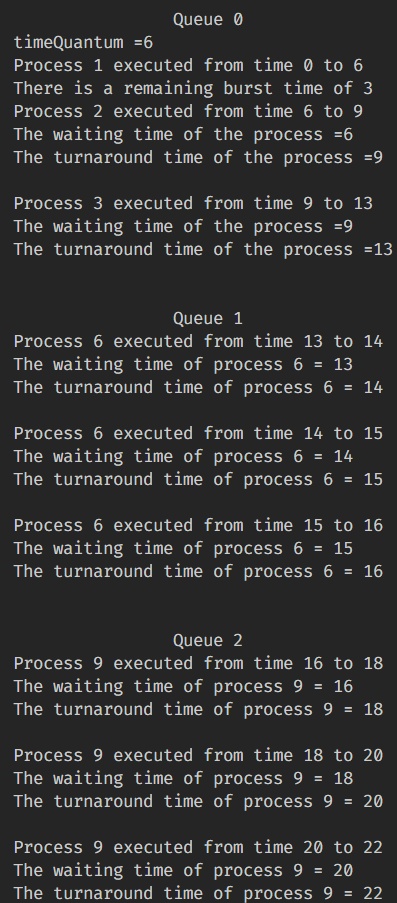
\includegraphics[width=\textwidth]{5.png}
    \caption{Queue 1}
    \label{fig:queue1}
  \end{subfigure}
  \hfill
  \begin{subfigure}[b]{0.45\textwidth}
    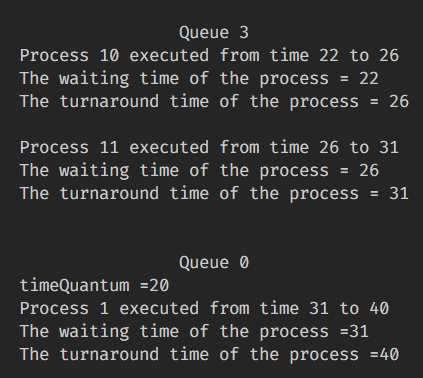
\includegraphics[width=\textwidth]{6.png}
    \caption{Queue 2}
    \label{fig:queue2}
  \end{subfigure}
  \caption{Code output}
  \label{fig:both_queues}
\end{figure}

\clearpage
\newpage
\section{Conclusion}
\subsection{Round Robin Scheduling Algorithm}
\begin{itemize}
  \item Setting the quantum too short produces the worst results, it increases the overhead.
  \item Higher average turnaround time than than SJF but better response.
  \item Turnaround time heavily depends on time quantum. It decreases if majority of burst time is lesser than the time quantum.
  \item Can be used for batch processing in multilevel queue.
  \item No starvation
\end{itemize}

\subsection{Shortest Job First Scheduling Algorithm}
\begin{itemize}
  \item Produces the optimal average turnaround time among these scheduling algorithms.
  \item If shorter jobs keep getting enqueued then aging has to be implemented to prevent starvation.
  \item Turnaround time heavily depends on time quantum. It decreases if majority of burst time is lesser than thetime quantum.
  \item Cannot be implemented at the level of short-term CPU scheduling.
  \item Can be used for interactive processing in multilevel queue.
\end{itemize}

\subsection{First In First Out Scheduling Algorithm}
\begin{itemize}
  \item Has low scheduling overhead because it does not require frequent context switches or involve complex scheduling decisions.
  \item Processes with shorter burst time will have to wait for an unreasonable time if processes with largest burst time arrive before it.
  \item Favours CPU bound processes than I/O bound processes.
  \item Perfect for processes with workloads with no strict time constraint.
  \item Can be used for system processing in multilevel queue.
\end{itemize}

\subsection{Multi Level Queue Scheduling Algorithm}
\begin{itemize}
  \item Overhead is low because the scheduler needs to only select the appropriate queue.
  \item Fairness is present in this algorithm.
  \item Processes in the lower levels face the starvation problem.
\end{itemize}

\section{Program Limitations}
The current version of the program assumes that all process arrivals occur at time 0. However, the program does not account for instances where processes can arrive at different times. This limitation prevents us from obtaining accurate results, such as waiting time and turnaround time, when different processes are enqueued at different times.

The quantum decision during the selection of the Round Robin time quantum has a significant impact. Choosing a static time quantum can lead to worse performance. Instead, we implemented a dynamic approach by using the time quantum from the multilevel queues. Although not perfect, this dynamic implementation produces better results compared to the static implementation.
When the Queue for round robin has more than 20 process only the first 20 process get 1 second to execute other process doesn't gets executed
\end{document}
